\documentclass[../../main.tex]{subfiles}
\begin{document}
\tracingall

Our algorithm is based on the two algorithms: two-scale Simulation \citep{solenthaler2011two} and regional time stepping \citep{goswami2014regional}. However, \citet{goswami2014regional} limited the research to WCSPH, while our algorithm only uses PCISPH. In an unpublished paper by Goswami and Batty, the RTS method is expanded for use with PCISPH. This is what we base our algorithm on. In this chapter we will explain these methods and why they improve the simulation times. More details can be found in the respective original papers, the unpublished RTS paper can be found in its fullness in Appendix A.

%%%%%%%%
\section{Two-scale simulation}
\label{sec:twoscale}
%%%%%%%%
The two-scale simulation technique, outlined in algorithm \ref{alg:twoscale}, uses two separate simulations to simulate a body of fluid, one high and one low resolution. The low resolution simulation, L-simulation or simply L, uses large particles and represents the entire simulation. The high resolution, H-simulation or H, on the other hand uses smaller particles and exist only as a subset of the L-simulation. 

By using larger, and thus fewer, particles for the entire simulation, as opposed to an equivalent simulation containing only high resolution particles, the total computational time is reduced. By identifying the regions where large particles fail to achieve the desired level of detail, we can make use of smaller particles to maintain visually pleasing results. Since the resolution of the particles in those regions is higher than the rest of the fluid, they are are called H-regions.

Identifying an H-region can be done with multiple approaches. It can be a predetermined region where a user has observed complex movement, like obstacles where collisions occur, see figure \ref{fig:complexarea}. Another option is to use dynamic approaches, such as using the view frustum, i.e. use larger particles for the part of the simulation that is currently not viewed by the observer. A third approach assumes that the visual results is most critical at the surface, which can be determined as the H-region using surface detection \citep{solenthaler2007efficient} and flood fill algorithm to expand downward from the surface.

\begin{figure}[h!]
    \centering
    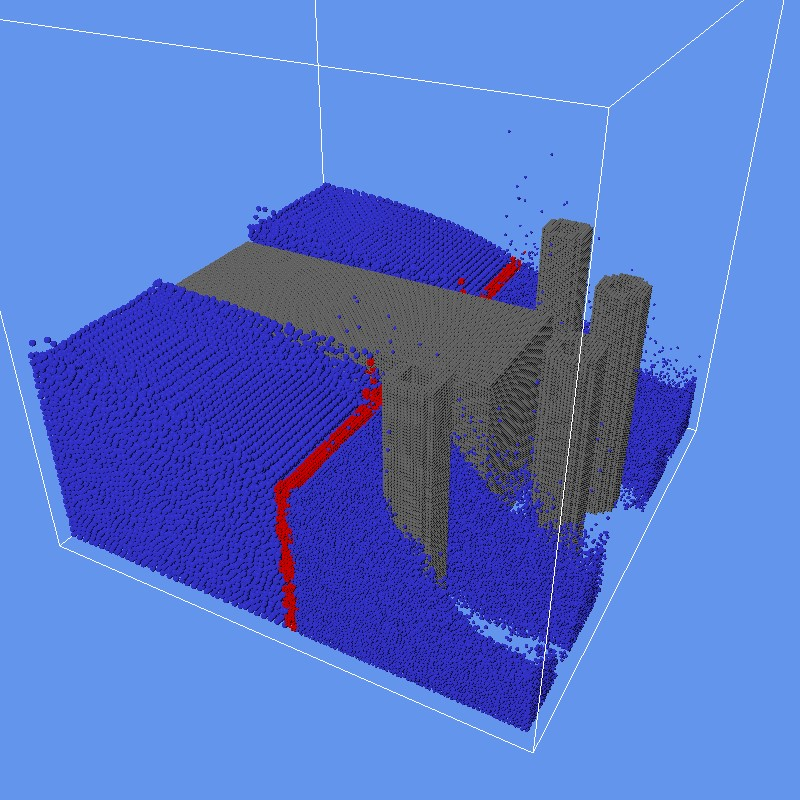
\includegraphics[width=\textwidth]{ComplexArea.jpg}
    \caption[Complex scene with user defined H-region]{A complex scene with a user defined H-region. The red particles represents the boundary region between the L and the H-region. Notice the particles in L (left) are larger than in H (right). The gray particles are static particles.
    }
    \label{fig:complexarea}
\end{figure}

Each particle in the H-simulation, referred to as an H-particle, has 1$/$\textit{n} the diameter of a particle in L, L-particle, where \textit{n} is the resolution factor and a multiple of 2. Due to instability risks introduced by using smaller particles which can more easily end up in physically incorrect positions, the H-simulation requires 1$/$\textit{n} the time step of the L-simulation. To prevent the H-simulation from lagging behind, we perform \textit{n} physics calculations and position forwarding for H every time step. 

Because the L-simulation acts as a base simulation and the H-simulation is an independent simulation, they need to be coupled so that the resulting fluids match. To tie the simulations together, a parent and children relationship is used. An H-particle has exactly one parent particle from L, which is computed by finding the closest L-particle. In contrast, an L-particle can have an unlimited number of children, but can only act as a parent as long as it occupies a position within the H-region. Only L-particles may act as a parent, and only H-particles may be created as children. 

When updating an H-particles parent and since a particle does not move very far each frame, checking its current parents neighbor for a closer particle typically suffices. If all particles in the neighborhood are farther away from the H-particle than a distance of an L-particles diameter, the whole L-simulation is searched for the closest particle. 

\begin{algorithm}[h]
    \caption{Two-Scale simulation}
    \label{alg:twoscale}
    \begin{algorithmic}[1]
        \While{animating}
        \State compute physics for \textit{L}
        \State determine regions in \textit{L}
        \State transfer region information from \textit{L} onto \textit{H}
        \State add / delete \textit{\texorpdfstring{H\textsubscript{boundary}}{H boundary}} particles
        \State interpolate quantities from \textit{L} onto \textit{\texorpdfstring{H\textsubscript{boundary, activeRelax}}{H boundary, activeRelax}}
        \For{\textit{nSubsteps}}
                \State compute physics for \textit{H}
            \State advect \textit{\texorpdfstring{H\textsubscript{boundary}}{H boundary}}
        \EndFor
        \State update parent particle in \textit{H}
        \State interpolate feedback information from \textit{{\texorpdfstring{H\textsubscript{active}}{H active}}} onto \textit{L}
        \EndWhile
   \end{algorithmic}
\end{algorithm}

A small area surrounding the H-region is defined as the boundary region. The boundary region is a critical part of the simulation because it is the only region where H-particles can be deleted or created. When an L-particle enters the boundary region from L, child particles are created to represent the parent within H. In contrast, if a parent leaves the boundary region and enters the L-region it deletes all associated children, see figure \ref{fig:boundary}. 

\begin{figure}[h!]
    \centering
    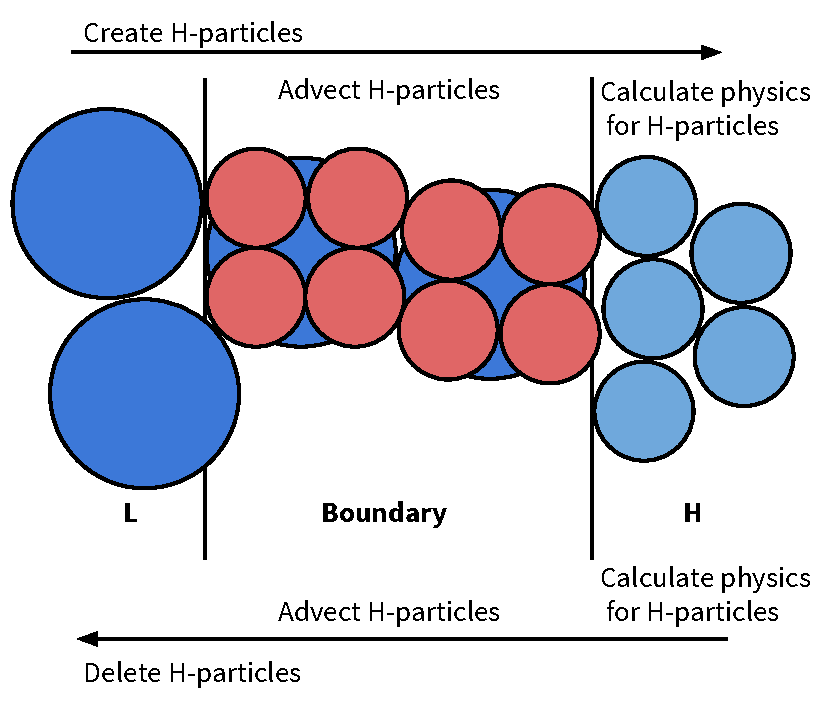
\includegraphics[width=\textwidth]{Two-scale-boundary.pdf}
    \caption[Two-scale H-region boundary handling]{ L-particles entering the boundary region of the H-region creates child particles in the H-simulation. These particles are advected until their parent exits the boundary region, they are then either deleted or set to the relaxed state, depending on the direction of the parent.  }
    \label{fig:boundary}
\end{figure}

It is important that all particles has a correct neighborhood for the physics calculations to be performed correctly. Since the H-particles are created at the edge of the H-region, they only have neighbors on one side and will be pushed out again. To counter this, the particles in the boundary region do not calculate neighborhoods or any physics. Instead the H-particles within the boundary region are advected by the flow of L until they are deleted or the parent enters the H-region. This way the H-particles in the H-region has a satisfying neighborhood along the boundary without losing the flow of the fluid. 

Furthermore, when a parent particle enters the H-region from the boundary region, its children enter what is called a relaxation period. This period exists because the particles coming from the boundary region may lie in a configuration which could cause sudden changes in density should they start physics calculations immediately. Therefore, the relaxed particles interpolate their quantities from advected values to physically correct values over a short period of time. 

The L-particles in the active region receive a feedback force from the smaller particles so that L and H do not diverge significantly. In addition, simulations with larger particles typically experience more dampening effects which is mitigated by the feedback from the smaller particles in the H-region. The feedback force is calculated from the average velocity of all children to each L-particle in the H-region. 

%%%%%%%%
\section{Regional time stepping}
%%%%%%%%
In conventional SPH methods, all regions of fluid are integrated with the same time step, even though different regions could actually be updated at different frequency depending on the velocities and forces in each region. With the assumption that small parts of a fluid are subject to approximately the same forces, Goswami and Batty discretizes the whole fluid domain into blocks. Each side of a block is twice as long as a particles diameter, thus a block can contain only a small number of particles. By giving each block a specific \textit{activity level} based on the forces and velocities of the containing particles, areas of the fluid with more rapid movement can be given more computational power (i.e. more calculations per animation frame) and regions with less movement can be given less, thus decreasing the total computational time. 

The activity levels are called regions and there are \textit{n} of them, $\Re_1$ to $\Re_n$, where $\Re_1$ is the region with highest force or velocity, as figure \ref{fig:rts} shows. A block is assigned the highest activity level, the lowest region number, for which it satisfies three equations based on the contained particles' maximum velocity, force, and the time step. For more detail about these equations we refer to \citet{goswami2014regional}.

\begin{figure}[h!]
    \centering
    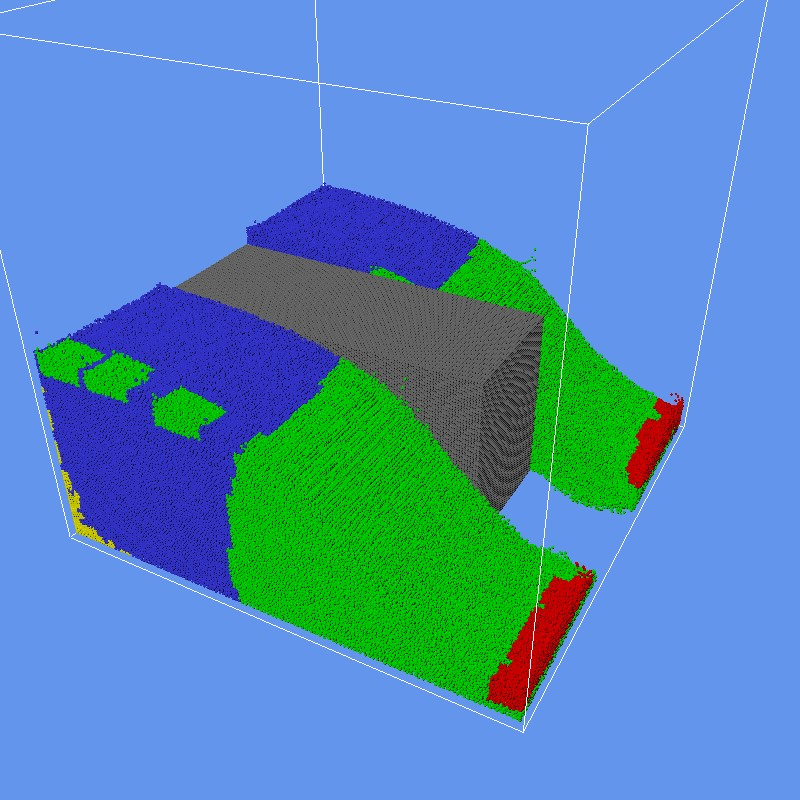
\includegraphics[width=\textwidth]{RTS.jpg}
    \caption[RTS on Double dam break]{ RTS simulation on the scene Double dam break. The regions are color coded as follows: $\Re_1$ red, $\Re_2$ green, $\Re_3$ blue, and $\Re_4$ yellow. $\Re_1$ occurs just as the particles are hitting the wall since much force is exerted on them from the wall. In contrast, the particles in the opposite corner belongs to $\Re_4$ since they are practically still.  }
    \label{fig:rts}
\end{figure}

% Major and minor steps
One animation frame is called a \textit{major step} and it consists of \textit{n minor steps}, where \textit{n} is the number of activity levels. Each minor step forwards the simulation $\Delta$t$_b$ seconds, the base time step, thus each major step is $n\Delta$t$_b$ seconds long. The idea is that some computations only need to be calculated once every major step, instead of every minor step. The neighborhood grid update, usually one of the most expensive parts of the PCISPH algorithm, is an example \citep{solenthaler2011two}. 

Particles in $\Re_1$ and $\Re_2$ could have such velocities that they travel outside their blocks over one time step, therefore, those regions are expanded 4 layers of blocks.

\begin{figure}[h!]
    \centering
    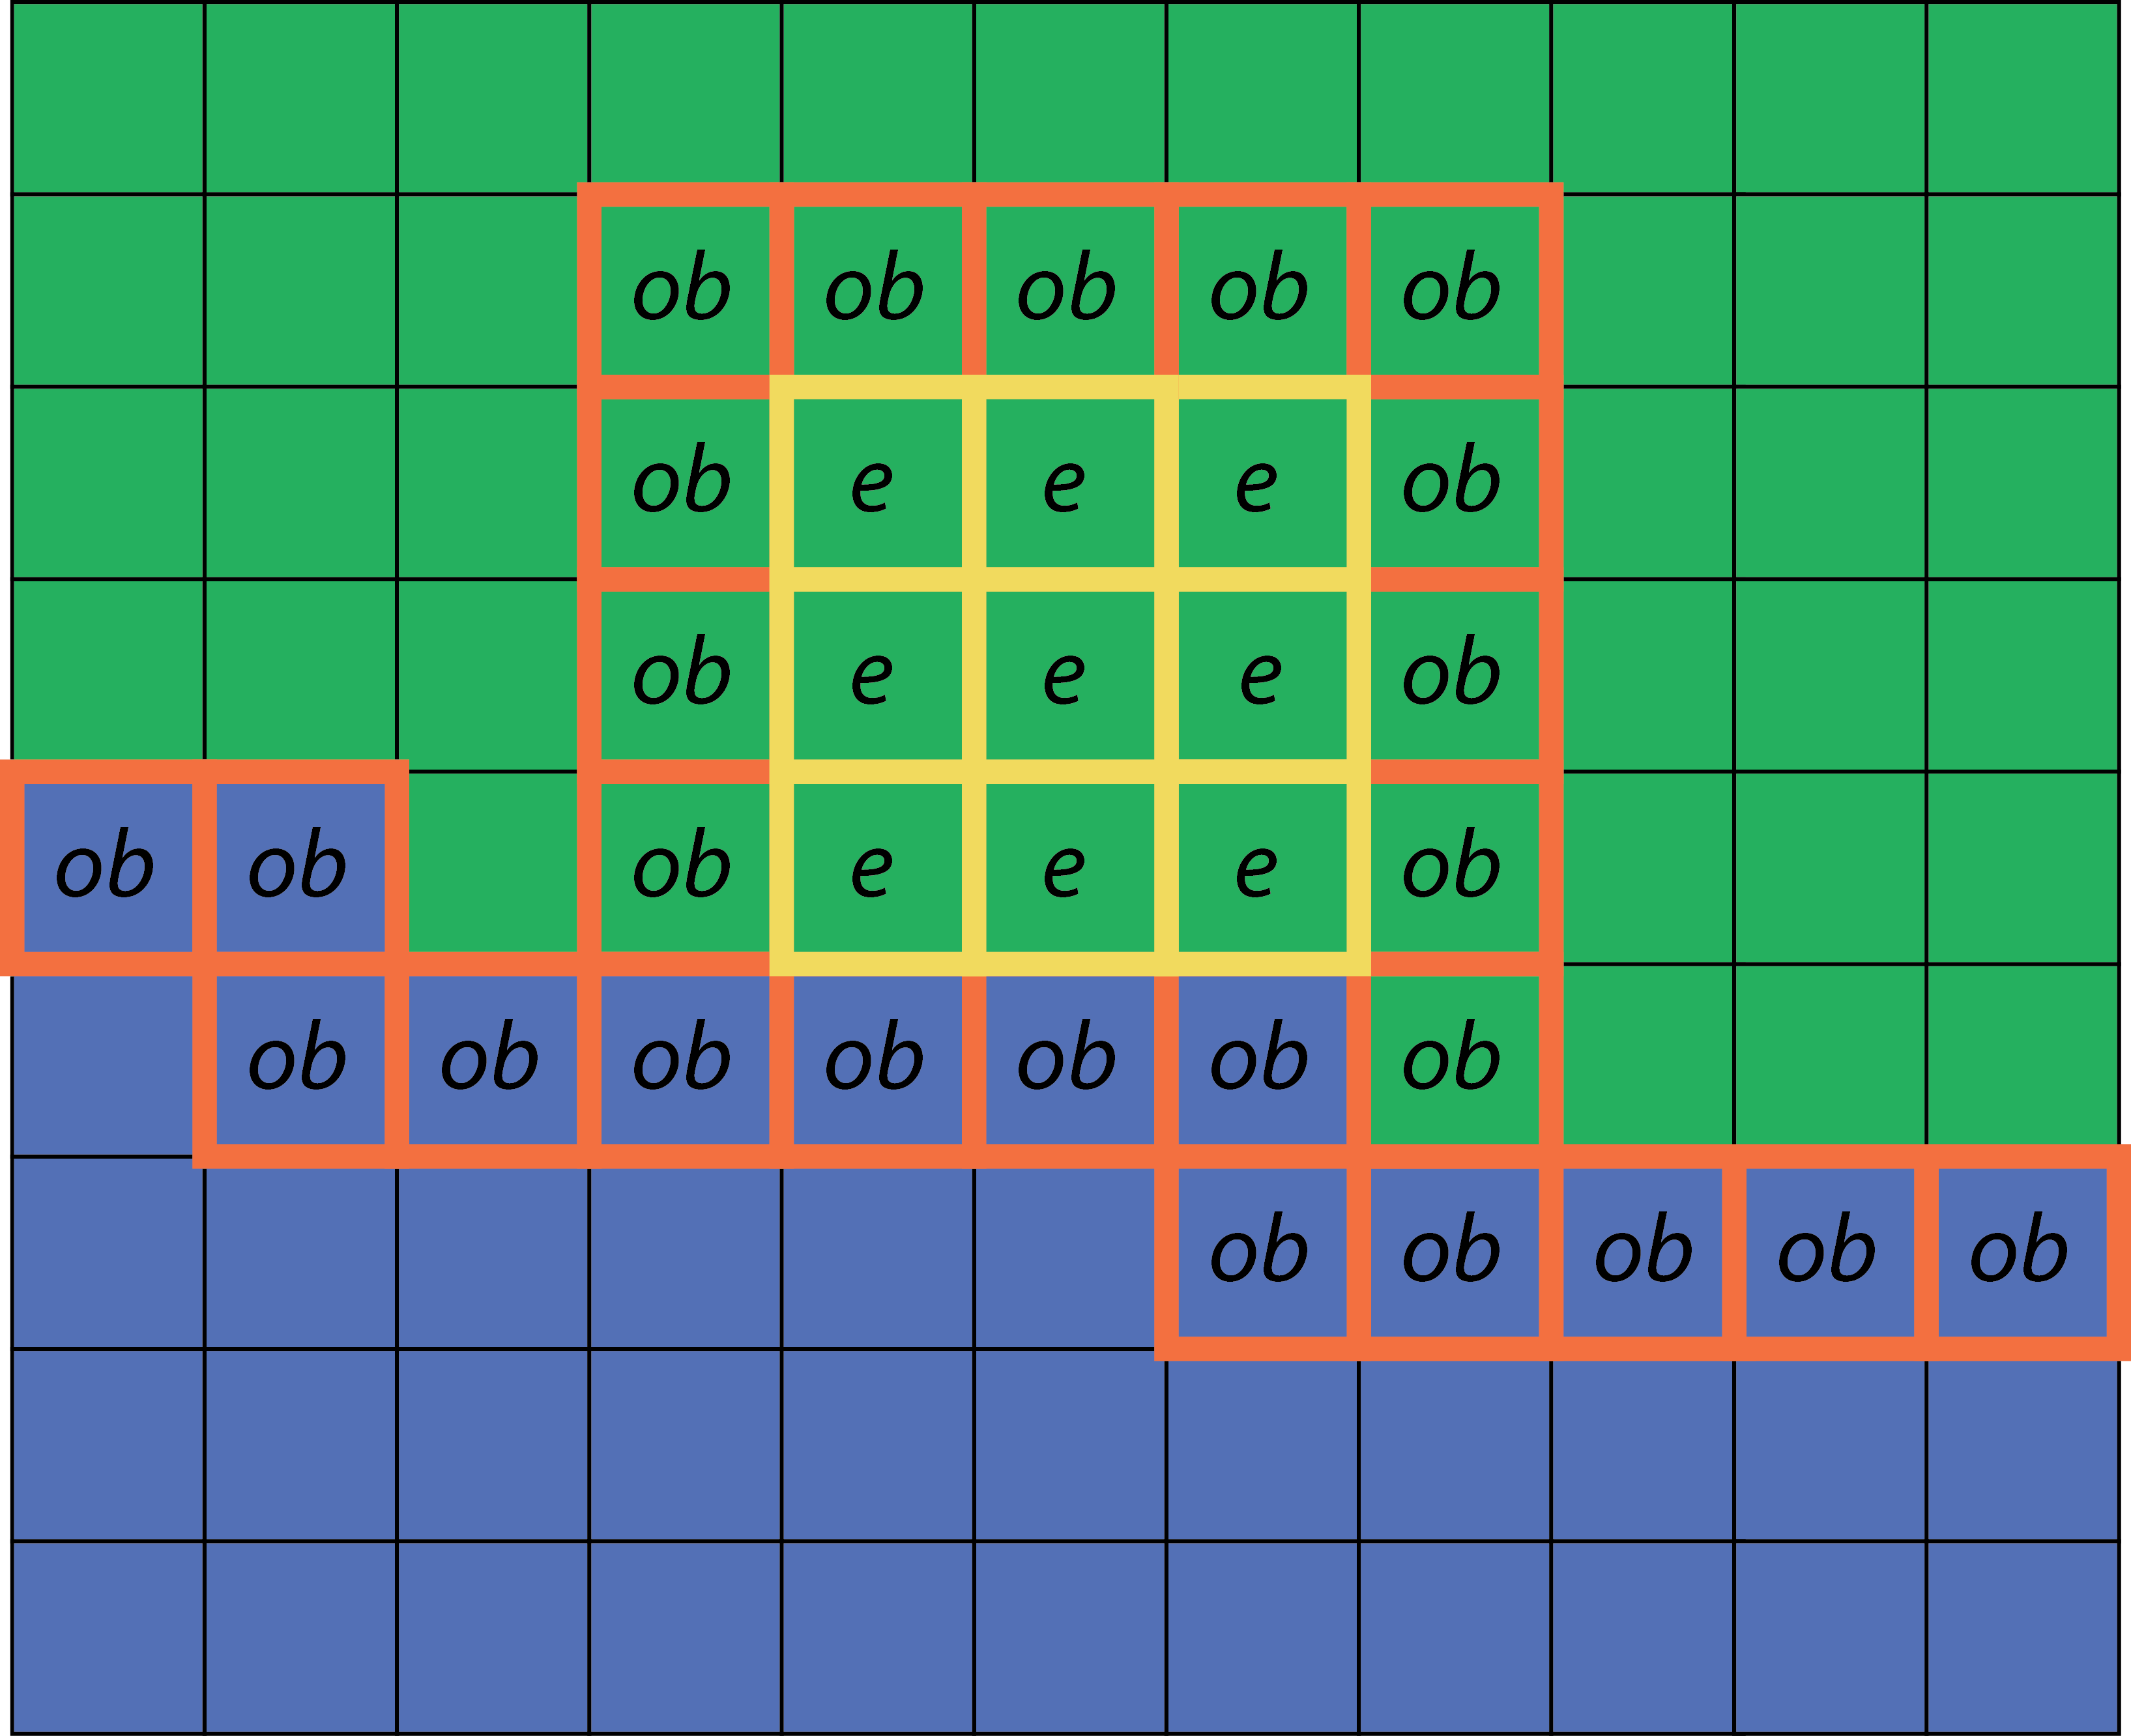
\includegraphics[width=\textwidth]{region_expansion.png}
    \caption[Region expansion for $R_x$]{ We use the same idea with region expansion and observed blocks $\Re_{ob}$ as in Goswamis extended paper, we mark blocks around erroneous blocks and region borders as observed. }
    \label{fig:region_exp}
\end{figure}

In addition, blocks bordering higher activity level blocks are marked as \textit{observed} blocks, $\Re_{ob}$, which are checked for density errors whenever the bordering region is corrected, as can be seen in figure \ref{fig:region_exp}. This way we only have to check the density of blocks neighboring the erroneous blocks since they are the only ones in risk of becoming erroneous themselves. 

% Conditional updates and toCompute
Inside the minor steps, all physics computations is made, however, since slow moving particles probably have the same neighborhood for an entire major step it does not need to be re-computed every minor step. On the other hand, faster moving particles will need to keep their neighborhood and densities updated. We keep track of which particles should be updated using the variables \textit{compute} and \textit{validity} for each particle. Before the minor steps we set \textit{compute} to true and \textit{validity} to the particles activity level. The \textit{validity} variable is decremented each minor step and \textit{compute} is updated according to algorithm \ref{alg:validity}. In algorithm \ref{alg:rts:pcisph}, \textit{conditional} means that a particle will only update if its \textit{compute} variable is set to true. 

\begin{algorithm}[]
    \caption{RTS for PCISPH}
    \label{alg:rts:pcisph}
    \begin{algorithmic}[1]
        \While{animating}
            \State update block neighborhood grid
            \State find max velocity \textit{v} and force \textit{F} per block
            \State calculate block activity level
            \State expand region $\Re_1$, $\Re_2$
            \State find observed block $\Re_{ob}$
            \For{\textit{nRTSMinorSteps}}
                \State conditional update neighborhood
                \State conditional update density $\rho$
                \State conditional update external forces \textbf{\textit{F}}$^{ext}$
                \State reset pressure \textit{p} and pressure forces \textbf{\textit{F}}$^p$
                \State prediction correction step (Algorithm \ref{alg:rts:correction})
                \State logic for half/full major step
                \State update velocity \textbf{\textit{v}} and position \textbf{\textit{x}}
                \State update validity (Algorithm \ref{alg:validity})
            \EndFor
        \EndWhile
   \end{algorithmic}
\end{algorithm}


% Prediction correction loop
Seeing as the regions with low velocity and forces do not change the particle density rapidly, the number of iterations they require in the correction loop is lower than the amount the higher activity levels need. Therefore, the particles are corrected according to algorithm \ref{alg:rts:correction} and the scheme in figure \ref{fig:schedule}, where \textit{e} denotes blocks that could not be corrected previous iteration, and will be corrected regardless of region membership. 

\begin{figure}[h!]
    \centering
    
\includegraphics[width=\textwidth]{schedule.png}
    \caption[Correction scheme for RTS]{ The density correction schedule used defined by Goswami and Batty in their unpublished paper. When read from left to right one can view the four minor steps, read from top and down we see the iteration within each minor step. In the first iteration within the first minor step all four regions $\Re_1$ ... $\Re_4$ performs prediction correction steps. It is designed so that each region performs at least one density correction each minor step. After the first iteration within a minor step we perform an iteration for $\Re_x$ if x modulus of the current minor step equals zero. However, $\Re_4$ is omitted in the fourth minor step as it made no impact on the visual results. Regions with fast moving particles receive more correction each minor step. }
    \label{fig:schedule}
\end{figure}

% Half/full major step
If some density error remains after the first 3 iterations, local corrections are performed on the blocks still marked as erroneous. If the average density error of the whole fluid is larger than a threshold, however, additional corrections are performed on all blocks. Should the correction loop fail to converge for a total of 6 iterations, the time step for the major steps is reduced to half, that is \textit{n}/2 $\Delta$t$_b$, because the neighbor grid update will happen more often and the simulation can therefore handle sudden density changes better. The time step is changed back to \textit{n}$\Delta$t$_b$ if the simulation has run 10 major steps with all correction loops exiting with every blocks density corrected. 

 
\begin{algorithm}[h]
    \caption{Update validity}
    \label{alg:validity}
    \begin{algorithmic}[1]
        \ForAll{\textit{i $\in$ particles}}
            \State decrement validity
            \If {validity$_i$ $\leq$ 0}
                \State set \textit{{\texorpdfstring{compute\textsubscript{i}}{compute i}}} = true
                \State update \textit{{\texorpdfstring{validity\textsubscript{i}}{validity i}}}
            \Else
                \State \textit{{\texorpdfstring{compute\textsubscript{i}}{compute i}}} = false
            \EndIf
        \EndFor
   \end{algorithmic}
\end{algorithm}


\begin{algorithm}[h]
    \caption{Density Correction RTS}
    \label{alg:rts:correction}
    \begin{algorithmic}[1]
        \While{iter $\leq$ minIterations || density$_{error}$ $\geq$ max density$_{error}$}
            \State predict velocity \textbf{\textit{v}} and position \textbf{\textit{x}}
            \State predict density $\rho$ and pressure \textit{p}
            \If{density error $\rho_{err}$ remains outside active regions}
                \State update $\Re_{err}$ and $\Re_{ob}$
            \EndIf
            \If{particle has turn}
                \State compute pressure force \textbf{\textit{F}}$^p$
            \EndIf
            \State iter++
            \If{$\rho_{err}$ $\geq$ max $\rho_{err}$ \& iter $\geq$ 3}
                \State minIterations++
                \If{$\rho_{err}$ $\geq$ density threshold}
                    \State perform extra global corrections
                \Else
                    \State perform local corrections on $\Re_{err}$
                \EndIf
            \EndIf
        \EndWhile
   \end{algorithmic}
\end{algorithm}

\end{document}